\section{Lezione 4}%
\label{sub:Lezione 4}
\subsection{Continuità dei processi stocastici}%
\label{sub:Continuità dei processi stocastici}
\begin{defn}[Processo continuo]
    Un processo stocastico si dice continuo se $\forall \epsilon > 0$: 
    \[
	\lim_{\Delta t \to 0} \frac{1}{\Delta t}\int\limits_{\Sigma_\epsilon}   dx_1 P_{1|1}(x_1, t + \Delta t | x_2, t) = 0
    .\] 
    \[
        \Sigma_\epsilon : \left\{ \left|x_1-x_2\right|>\epsilon\right\}
    .\] 
\end{defn}
\noindent
In pratica serve che il cammino descritto dal processo sia continuo, la distanza tra due punti del processo deve andare a $0$ più rapidamente di $\Delta t$.\\
I processi Markoviani non sono necessariamente continui:
\begin{exmp}[Pollaio]
    Il numero di uova prodotte in un pollaio in un giorno può essere schematizzato come processo markoviano: dipende soltanto dal numero di galline presenti nel pollaio il giorno prima.\\
    Questo processo non può essere continuo: è possibile mandare il $\Delta t$ a $0$ ma non possiamo fare altrettanto con $x$, ovvero il numero di uova. Infatti in questo caso il numero di uova è discreto. \\
    In generale i processi a salti discreti non possono essere continui.
\end{exmp}
\noindent
\begin{exmp}[Moto Browniano]
    Calcoliamo l'equivalente della $P_{1|1}$ nel moto Browniano, nella lezione $1$ abbiamo visto che:
    \[
	P(x, t+\Delta t) = \int P(x-\Delta, t) f(\Delta) d\Delta
    .\] 
    Con $f(\Delta)$: probabilità di fare un salto lungo $\Delta$ nell'intervallo di tempo $\Delta t$.\\
    Definendo la quantità $y = x-\Delta$ intuitivamente la $f(\Delta)$ corrisponde alla probabilità condizionata:
    \[
	f(\Delta) = P_{1|1}(x, t+\Delta t| y, t) 
    .\] 
    Essendo un oggetto Gaussiano la $f(\Delta)$ avrà la seguente struttura:
    \[
	f(\Delta) = \frac{1}{\sqrt{4\pi D\Delta t} }\exp\left(-\frac{1}{4D\Delta t} \left(x-y\right)^2  \right) 
    .\] 
    In altre parole $f(\Delta)$ è proprio un propagatore.\\
    Inserendo questo oggetto nella definizione di processo continuo si vede che l'uguaglianza al limite è soddisfatta, quindi il moto Browniano è un processo continuo.
\end{exmp}
\noindent
\begin{exmp}[Moto di Cauchy]
    Il moto di Cauchy presenta una struttura per la probabilità di salto (condizionata) del seguente tipo:
    \[
	P_{1|1}(x,t+\Delta t| z , t)  = \frac{\Delta t}{\pi} \frac{1}{\left(x-z\right)^2 + \left(\Delta t\right)^2}
    .\] 
    E si può dimostrare che:
    \[
	\lim_{\Delta t \to 0} \frac{1}{\Delta t}\int\limits_{\Sigma_\epsilon}
	\frac{\Delta t dx}{\pi\left[\left(x-z\right)^2 + \left(\Delta t\right)^2\right]} = \infty
    .\] 
    Di conseguenza il moto di Cauchy non è continuo.
\end{exmp}
\noindent
\begin{figure}[H]
    \centering
    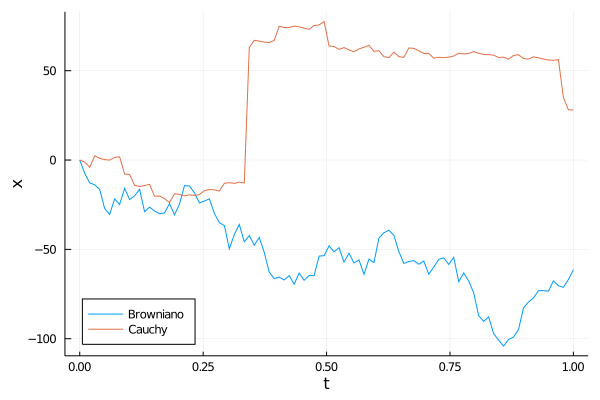
\includegraphics[width=0.4\textwidth]{figures/4_cauchy-brown.png}
    \caption{\scriptsize Processo di Brown e Processo di Cauchy a confronto (Ottenuto in Julia).}
    \label{fig:-fig}
\end{figure}

%%%%%%%%%%%%%%%%%%
%  Chapman form  %
%%%%%%%%%%%%%%%%%%

\subsection{Forma differenziale di Chapman - Kolmogorov}%
\label{sub:Forma differenziale di Chapman - Kolmogorov}
Prendiamo un processo stocastico scomponibile\
\footnote{Ipotesi per cui si può scomporre sul Gardiner}  in una parte continua ed una non continua.\\
Si può dimostrare che un processo di questo tipo è descritto dalla seguente forma differenziale:
\begin{redbox}{Forma di Chapman-Kolmogorov}
 \[
    \partial_{t}P(\vect{z},t| \vect{y}, t') = - \Gamma + \Phi
.\]    
\end{redbox}
\noindent
In cui $\Gamma$ è la parte contenente il processo continuo:
\[\begin{aligned}
    \Gamma = \sum_{i}^{} \partial_{z_i}&\left[ A_i(\vect{z},t) P(\vect{z},t|\vect{y},t') \right] +\\
                         &+\sum_{i,J}^{} \frac{1}{2}\partial^2_{z_iZ_J}\left[ B_{iJ}(z,t) P(\vect{z},t|\vect{y},t') \right]
.\end{aligned}\]
Qui abbiamo un primo termine "deterministico" (con la $A$) che determina soltanto uno spostamento dell'oggetto ed un termine di diffusione (quello in $B$).\\
Nella $\Phi$ abbiamo invece il processo discontinuo:
\[\begin{aligned}
    \Phi = \int  d\vect{x} &\left[\omega (\vect{z}|\vect{x}, t) P(\vect{x},t|\vect{y}, t') \right. + \\
			   & \left. - \omega(\vect{x} | \vect{z}, t)  P(\vect{z},t|\vect{y},t') \right]
.\end{aligned}\]
Il termine $\Phi$ somiglia molto al termine della equazione di Volterra che abbiamo visto nella prima lezione (prob. di trovarsi in $\vect{z}$ è data dalla probabilità di finire in $\vect{z}$ da una posizione $\vect{x}$ diminuito la prob. di scappare in $\vect{x}$ dalla posizione $\vect{z}$).\\
La potenza della equazione è la sua generalità: se sappiamo che un processo è Markoviano (magari per la fisica che ci sta dietro) allora l'equazione di evoluzione delle prob. nel tempo sarà necessariamente quella sopra.
\begin{exmp}[$A=B=0$, quindi $\Gamma =0$]
    \[
        \partial_{t}P = \Phi
    .\] 
    Considerando il rapporto incrementale con passo $\Delta t$:
    \[
	P(z, t+\Delta t|y, t) = P(z,t|y,t) + \Delta t\cdot  \Phi
    .\] 
    Sfruttiamo la proprietà ovvia:
    \[
	P(\vect{z}, t|\vect{t}, t) = \delta (\vect{y}-\vect{z}) 
    .\] 
    Allora possiamo sviluppare l'espressione con $\Delta t$ che tende a $0$ (mettiamoci in una dimensione per semplicità):
    \begin{greenbox}{Soluzione della forma diff. con termini continui}
    \[\begin{aligned}
	P&(z, t + \Delta t| y, t) = \\
				  &= \delta (z-y) \left[1-\Delta t\int dx \omega (x|z) \right] + \Delta t \cdot \omega (z|y) 
    .\end{aligned}\]
    \end{greenbox}
    \noindent
\end{exmp}
\noindent

\subsection{Processo di Wiener}%
\label{sub:Processo di Wiener}
Un processo di Wiener è modellato dalla seguente equazione:
\begin{greenbox}{Equazione per processo di Wiener}
    \[
	\frac{\partial }{\partial t} P(\omega,t|\omega_0, t_0) =
	\frac{1}{2}\frac{\partial ^2}{\partial \omega^2} P(\omega, t|\omega_0, t_0) 
    .\] 
\end{greenbox}
\noindent
Inoltre deve esser rispettata la condizione iniziale:
\[
    P(\omega,t_0|\omega_0, t_0) = \delta (\omega-\omega_0) 
.\]
Il processo si può risolvere utilizzando la funzione caratteristica:
\[
    \phi (s, t) = \int d\omega P(\omega, t|\omega_0, t_0) e^{is\omega}
.\] 
Sfruttando le regole della trasformata possiamo riscrivere l'equazione del processo come:
\[
    \frac{\partial \phi }{\partial t} = -\frac{1}{2}s^2\phi
.\] 
\[
    \phi (s, t_0) = \exp (is\omega_0) 
.\] 
La soluzione è nota:
\[\begin{aligned}
    \phi (s) =& \exp\left(-\frac{1}{2}s^2\left(t-t_0\right)\right)\phi (s,t_0)  =\\
    	=&\exp\left(-\frac{1}{2}s^2\left(t-t_0\right) + is\omega_0 \right) 
.\end{aligned}\]
Visto che l'antitrasformata di una Gaussiana è una Gaussiana abbiamo la soluzione nello spazio reale:
\begin{redbox}{Soluzione del processo di Wiener}
    \[
	P(\omega,t|\omega_0, t_0) = 
	\frac{1}{\sqrt{2\pi\left(t-t_0\right)} }
	\exp\left(- \frac{\left(\omega-\omega_0\right)^2}{2\left(t-t_0\right)}\right)
    \] 
\end{redbox}
\noindent
Il processo che abbiamo ottenuto è Gaussiano:
\[
    \left<\omega\right> =  \omega_0
.\] 
\[
    \left<\left(\omega-\omega_0\right)^2\right> = t- t_0
.\] 
\paragraph{Proprietà dei processi di Wiener}%
\label{par:Proprietà dei processi di Wiener}
\begin{itemize}
    \item \'E continuo.
    \item Non è differenziabile, $\forall k$:
	\[\begin{aligned}
	    \text{Prob}&\left(\frac{\left|\omega (t+h) - \omega (t) \right|}{h}> k\right) = \\
		       & = 2 \int_{kh}^{\infty} d\omega  \frac{1}{\sqrt{2\pi  h}} e^{- \omega^2 /2h} 
		       \ \xrightarrow[]{h\to 0} 1
	.\end{aligned}\]
    \item Gli incrementi sono indipendenti:
	\[\begin{aligned}
	    P(&\omega_2, t_2; w_1,t_1; \omega_0,t_0) = \\
	      &= P(\omega_2, t_2|\omega_1,t_1) P(\omega_1, t_1|\omega_0,t_0) P(\omega_0,t_0) 
	.\end{aligned}\]
	Il primo termine dopo l'uguale non dipende da $(\omega_0,t_0)$ perché il processo è Markoviano.
    \item La correlazione: 
    \[
	\left<\omega (t) \omega (s) | \left[\omega_0, t_0\right]\right> = \text{min}(t-t_0, s-s_0) + \omega_0^2
    .\] 
    Che nel caso particolare in cui $\omega_0=t_0=0$ si ha $\left<\omega (t) \omega (s) \right> = s$ se $t>s$.
    \usetikzlibrary{math}
    \tikzmath{\x = 5; \y = 4;}
    \begin{center}
    \begin{tikzpicture}
	 \draw[-stealth] (0,0) --(\x/\y, 0)node[below]{$s$} -- (\x,0) node[right]{$t$};
	 \draw[-stealth] (0,0) --(0,\x/\y)node[left]{$s$} -- (0,\x*2/5) node[above]{$\left<\omega (t) \omega (s) \right>$};
         \draw[thick] 
		  (0,0) node[below]{$0$} -- 
		  (\x/\y,\x/\y)  -- 
		  (\x,\x/\y);
	 \draw[dash dot] 
		  (\x/\y, 0) --
		  (\x/\y, \x/\y);
	\draw[dash dot] 
		  (0,\x/\y) --
		  (\x/\y, \x/\y);

    \end{tikzpicture}
    \end{center}
    \noindent
\end{itemize}
\clearpage
